\documentclass{article}

\usepackage{neurips_2026}
\usepackage[utf8]{inputenc}
\usepackage[T1]{fontenc}
\usepackage[american]{babel}
\usepackage{hyperref}
\usepackage{url}
\usepackage{graphicx}
\usepackage{mathtools}
\usepackage{amssymb}
\usepackage{booktabs}
\usepackage{nicefrac}
\usepackage{microtype}
\usepackage{xcolor}

\bibliographystyle{plainnat}
\renewcommand{\bibsection}{\section*{References}}

%% Macros
\newcommand{\crps}{\mathrm{CRPS}}
\newcommand{\crpss}{\mathrm{CRPSS}}
\newcommand{\dss}{\mathrm{DSS}}
\newcommand{\mse}{\mathrm{MSE}}
\newcommand{\rmse}{\mathrm{RMSE}}
\newcommand{\R}{\mathbb{R}}
\newcommand{\E}{\mathbb{E}}
\newcommand{\Var}{\mathrm{Var}}
\newcommand{\Norm}{\mathcal{N}}
\newcommand{\dd}{\mathrm{d}}
\DeclareMathOperator*{\argmin}{arg\,min}
\newtheorem{lemma}{Lemma}
\newtheorem{proposition}{Proposition}

\title{Fast Tree-Based Diffusions and Flows for Probabilistic Tabular Regression}

\author{Anonymous Authors}

\begin{document}
\maketitle

\begin{abstract}
We extend Treeffuser, a score-based diffusion model for probabilistic tabular regression with gradient-boosted trees, by treating regression conditioning as the central design axis. On the score side, conditional-mean residualization, EDM-style preconditioning, log-sigma time sampling, and noise-level features make the denoising regression better matched to histogram-split tree learners. On the flow side, Gaussian-path flow matching gives a directly learned velocity field with algebraic score recovery, enabling both few-step deterministic ODE sampling and stochastic-interpolant diagnostics. Across ten UCI benchmarks with fold-0 tuning and folds-1--5 evaluation, the score-side recipe gives the best Treeffuser calibration, reducing 95\% coverage error from 0.023 to 0.015 and cutting sampling time 6.5$\times$ over the published baseline. The FM row gives the best normalized CRPS among Treeffuser rows and is another 2.4$\times$ faster than the improved score model, but gives back some coverage. These are Pareto improvements rather than decisive dominance: gains over the published baseline are directional rather than conventionally significant ($p \approx 0.07$), and tuned non-diffusion baselines still win several datasets on raw CRPS. Stochastic ($\varepsilon > 0$) samplers do not Pareto-dominate the deterministic corner, so the empirical recommendation is $\varepsilon = 0$ when aggregate CRPS and latency are the target, while stochasticity remains a conditional-tail calibration knob.
\end{abstract}

\section{Introduction}\label{sec:intro}
Probabilistic regression on tabular data must combine the predictive strength of gradient-boosted trees with full predictive distributions usable for calibration, decision-making, and uncertainty quantification. Treeffuser~\citep{treeffuser} achieves this by training LightGBM~\citep{ke2017lightgbm} regressors to estimate the score of a noise-perturbed conditional density and integrating the corresponding reverse-time stochastic differential equation (SDE)~\citep{song2021score} at inference. The framework inherits the calibration properties of score-based diffusion while avoiding neural-network density estimators.

Our notion of tractability is computational rather than likelihood-exact: predictive quantities are Monte Carlo estimates, but training reduces to supervised tree regression, the final FM row samples with a five-step Heun ODE, and Eq.~\eqref{eq:score} recovers scores when stochastic sampling is desired.

We develop Treeffuser along two axes: score-side modifications matched to histogram-bin tree learners, and Gaussian-path flow matching~\citep{lipman2023flow,liu2023rectified}, which removes the indirect score-to-drift mapping and opens access to stochastic interpolants~\citep{albergo2023stochastic} with non-negative stochasticity schedule $\varepsilon(t)$.

\paragraph{Contributions.} We make three contributions:
\begin{enumerate}
  \item \emph{Score-side modifications for tree-based diffusion:} conditional-mean residualization, EDM preconditioning, log-$\sigma$ time sampling, and an explicit log-$\sigma$ feature for LightGBM score regression (\S\ref{sec:score-side}).
  \item \emph{Flow matching for Treeffuser:} a Gaussian-path FM trainer with score recovery when stochastic-interpolant sampling or endpoint-error analysis requires it (\S\ref{sec:fm}, Lemma~\ref{lem:wronskian-score}).
  \item \emph{Regression-conditioning unification:} regression conditioning for the tree ensemble as the bottleneck behind both score- and flow-side gains (\S\ref{sec:disc}, Appendix~\ref{app:theory}).
\end{enumerate}

Across ten UCI benchmarks, with one fold for tuning and five for evaluation, the score-side recipe gives the best aggregate calibration and CRPS skill score among Treeffuser rows, while FM gives the best aggregate normalized CRPS and fastest Treeffuser sampler. The shared lesson is that noising path, parameterization, training distribution, features, and sampler must make the induced supervised problem well matched to histogram splits.

\section{Method}\label{sec:method}

\subsection{Score-Side Modifications}\label{sec:score-side}
The published Treeffuser uses VESDE marginals with uniform $t$ sampling, a noise-prediction target, and LightGBM features $[\,y_t,\,X,\,t\,]$. We change four pieces: response/input conditioning, allocation of training rows over noise levels, explicit noise-level features, and sampler efficiency.

\paragraph{Conditional-mean residualization.} We fit a cross-validated LightGBM mean predictor $\hat{\mu}(x)$ and apply diffusion to $y - \hat{\mu}(x)$ rather than $y$, moving conditional location out of the score-regression target. The residualizer uses a high-capacity configuration selected from a prior diagnostic sweep (Appendix~\ref{app:resid-config}) and then fixed; it is not tuned jointly with the diffusion or flow hyperparameters. On large datasets this fixed residualizer can become a bottleneck once the inner model has enough data to represent the conditional mean directly.

\paragraph{EDM preconditioning.} Following \citet{karras2022edm}, we predict a denoised target $D_\theta(y_t, t)$ scaled to unit variance across noise levels and reconstruct the score $s(y_t, t) = (D_\theta - y_t)/\sigma(t)^2$. This stabilizes the regression target for trees, which would otherwise need to extrapolate noise-prediction magnitudes across $t$.

\paragraph{Log-sigma time sampling.} We draw $\log\sigma(t) \sim \Norm(-1.2, 1.2^2)$, clip to the SDE's achievable range, and invert. Because trees bin features by data density, the training-time distribution directly controls where the score model spends capacity.

\paragraph{Log-sigma noise feature.} The feature vector for LightGBM becomes $[\,y_t,\,X,\,t,\,\log\sigma(t)\,]$, giving the regressor an explicit noise-level signal aligned with EDM scaling.

\subsection{Flow Matching with Gaussian Paths}\label{sec:fm}
A Gaussian flow path interpolates data $y_0$ and a standard-normal prior $z$ via
\begin{equation}\label{eq:path}
y_t = \alpha(t)\, y_0 + \beta(t)\, z, \quad t \in [0,1],
\end{equation}
with boundary conditions $\alpha(0)=1$, $\alpha(1)=0$, $\beta(0)=0$, $\beta(1)=1$. We compare three paths: \emph{linear} ($\alpha = 1-t$, $\beta = t$), \emph{trigonometric} ($\alpha = \cos(\pi t/2)$, $\beta = \sin(\pi t /2)$), and a \emph{VP} schedule with linear $\beta_t$ giving $\alpha^2(t) = \exp(-T(t))$, $T(t) = \tfrac{1}{2}\beta_{\min} t + \tfrac{1}{4}(\beta_{\max} - \beta_{\min}) t^2$. The training target is the conditional velocity $u_t = \alpha'(t) y_0 + \beta'(t) z$, regressed against the model's $v_\theta(y_t, x, t)$.

\paragraph{Velocity-to-score formula.} For any Gaussian path with Wronskian $W(t) = \alpha(t) \beta'(t) - \alpha'(t) \beta(t)$, the conditional score is algebraically recoverable from the population velocity:
\begin{equation}\label{eq:score}
\nabla \log p_t(y_t \mid x) \;=\; \frac{\alpha'(t)\, y_t - \alpha(t)\, v_\theta(y_t, x, t)}{W(t)\,\beta(t)}.
\end{equation}
For linear FM this reduces to $-(y_t + (1-t) v)/t$; for trig to $-y_t - (2/\pi)\cot(\pi t/2) v$.
We use this identity operationally: it lets a velocity-trained Treeffuser enter the same stochastic-interpolant sampler family as score matching and exposes the endpoint amplification studied in Appendix~\ref{app:theory}.

\paragraph{Stochastic-interpolant family.} \citet{albergo2023stochastic} show that any non-negative $\varepsilon(t)$ defines a marginal-preserving reverse-time sampler at the population velocity/score:
\begin{equation}\label{eq:sde}
\dd y_\tau = \left(-v_\theta + \tfrac{\varepsilon^2}{2}\, s_\theta\right) \dd \tau + \varepsilon\, \dd W_\tau,
\end{equation}
where $\tau = 1 - t$ is reverse time and $s_\theta$ is the score from \eqref{eq:score}. The choice $\varepsilon \equiv 0$ recovers the deterministic probability-flow ODE; positive $\varepsilon(t)$ broadens samples, with exact marginal preservation only for the true velocity/score. We use the schedule $\varepsilon(t) = c\, t$, which vanishes at the data endpoint and suppresses recovered-score error in the stochastic drift (see Proposition~\ref{prop:endpoint-amp}).

\paragraph{Why these choices suit trees.} Eq.~\eqref{eq:score} makes FM compatible with stochastic-interpolant samplers; variance-preserving paths keep the tree input $y_t$ near unit scale, unlike a linear path with $\Var(y_t)\approx(1-t)^2+t^2$; and $\varepsilon=0$ avoids recovered-score error in the stochastic drift (Appendix~\ref{app:theory}). The path choice is therefore a finite-regression and sampler tradeoff, not a theorem that VP must dominate every tuned linear-flow row.

\subsection{Implementation Notes}\label{sec:impl}
The FM code reuses Treeffuser's per-output-dimension LightGBM fitter and feature pipeline; only the target and prior change. Sampling uses the same Heun integrator and residualizer as the score path, and both training and sampling avoid the singular endpoint with $t \geq 10^{-5}$.

\section{Experiments}\label{sec:exp}

\paragraph{Datasets and protocol.} Ten UCI benchmarks (Table~\ref{tab:per-dataset}) are evaluated with a nested tuning protocol. We split each dataset into six folds: fold~0 is used only for hyperparameter selection, and folds~1--5 are evaluation folds. For each dataset/model family, Optuna tunes on the fold-0 train/validation split; the selected configuration is then refit and evaluated on each held-out evaluation fold. Evaluation-fold training rows range from 256 on yacht to 38{,}108 on protein. For sample-based methods, each test point uses 200 samples; Treeffuser sampler choices are detailed in Appendix~\ref{app:datasets}. Metrics are averaged over evaluation folds and, for headline summaries, over datasets.

\paragraph{Metrics.} We report CRPS skill score $\crpss = 1 - \crps_{\text{model}} / \crps_{\text{climatology}}$, mean rel-CRPS, DSS~\citep{dawid1984pit}, PIT-KS pass rate at $\alpha=0.05$, absolute coverage error at 50/90/95\% nominal levels~\citep{gneiting2007crps}, and sample-generation time. CRPSS and rel-CRPS are the aggregate comparison metrics because raw CRPS is target-scale dependent; mean climatological CRPS ranges from 0.0043 on \texttt{naval} to 44.8 on \texttt{diabetes}. Timings are measured on one Apple-arm64 workstation, exclude fitting, and include generating 200 samples per test point plus inverse transformations. They use practical benchmark settings rather than a single-thread cap: Treeffuser samples in batches with \texttt{n\_parallel=20} and LightGBM \texttt{n\_jobs=-1}; other libraries use their configured parallel defaults.

\paragraph{Variants compared.} Three Treeffuser rows compare bundled recipes: (1)~\textsc{published}---the original baseline with noise-prediction, uniform $t$, no residualization; (2)~\textsc{score+}---the baseline plus \S\ref{sec:score-side}; (3)~\textsc{FM}---VP flow matching with residualization and a 5-step Heun ODE. Each row is tuned per dataset under the same fold-0 protocol. The residualizer-C configuration used in the headline rows was selected from the prior diagnostic sweep in Appendix~\ref{app:resid-config} and then fixed; it is not tuned jointly with the diffusion or flow hyperparameters. We also compare against six per-dataset tuned probabilistic baselines: NGBoost~\citep{duan2020ngboost}, quantile-regression LightGBM~\citep{ke2017lightgbm}, CatBoost RMSE-with-uncertainty~\citep{prokhorenkova2018catboost}, iBUG~\citep{brophy2022ibug}, a Gaussian deep ensemble~\citep{lakshminarayanan2017deep}, and CARD-style neural diffusion~\citep{han2022card}.

\begin{table*}[!t]
  \centering
  \caption{Headline real-data results, mean over 10 UCI benchmarks with fold~0 used for tuning and folds~1--5 used for evaluation. rel-CRPS is the per-dataset CRPS divided by the best displayed variant on that dataset. $|\text{cE}|$@$q$ is absolute coverage error at the $q$\% interval level. The CARD row is a compact benchmark adapter, not a fully optimized CARD pipeline (see Appendix~\ref{app:competitors}).}\label{tab:headline}
  \scriptsize
  \begin{tabular}{lrrrrrrr}
    \toprule
    Variant & CRPSS $\uparrow$ & rel-CRPS $\downarrow$ & KS $p{>}.05$ $\uparrow$ & $|\text{cE}|$@50 $\downarrow$ & $|\text{cE}|$@90 $\downarrow$ & $|\text{cE}|$@95 $\downarrow$ & samp.\ time \\
    \midrule
    Treeffuser-published & 0.670 & 1.242 & 0.40 & 0.117 & 0.044 & 0.023 & 221.35\,s \\
    Treeffuser-score$^+$ (ours) & \textbf{0.681} & 1.131 & \textbf{0.62} & 0.069 & \textbf{0.020} & \textbf{0.015} & 34.12\,s \\
    Treeffuser-FM (ours) & 0.680 & \textbf{1.117} & 0.46 & \textbf{0.064} & 0.028 & 0.024 & 14.41\,s \\
    \midrule
    QReg-LightGBM & 0.668 & 1.459 & 0.34 & 0.066 & 0.041 & 0.044 & 0.30\,s \\
    CatBoost-unc. & 0.638 & 1.409 & 0.28 & 0.093 & 0.078 & 0.066 & \textbf{0.01\,s} \\
    NGBoost & 0.601 & 1.550 & 0.16 & 0.119 & 0.114 & 0.101 & 0.04\,s \\
    Deep ensemble & 0.654 & 1.519 & 0.26 & 0.090 & 0.032 & 0.018 & 0.03\,s \\
    iBUG & 0.649 & 1.471 & 0.36 & 0.111 & 0.051 & 0.065 & 2.89\,s \\
    CARD-style diffusion & 0.631 & 1.632 & 0.24 & 0.086 & 0.057 & 0.043 & 42.84\,s \\
    \bottomrule
  \end{tabular}
\end{table*}

\subsection{Headline Result}\label{sec:headline}
Table~\ref{tab:headline} reports cross-dataset means under the tuning/evaluation protocol. The score-side recipe lifts CRPSS from 0.670 to 0.681, raises PIT-uniformity pass rate from 0.40 to 0.62, reduces 90/95\% coverage error from 0.044/0.023 to 0.020/0.015, and cuts Treeffuser sample time 6.5$\times$. FM is close on CRPSS, has the best aggregate normalized CRPS among displayed rows, and is another 2.4$\times$ faster than score$^+$, but gives back part of score$^+$'s coverage advantage. Per-dataset raw-CRPS winners span five families; a Treeffuser variant wins on 6/10 datasets, with the remaining wins split across deep ensembles, CARD-style diffusion, and quantile-regression LightGBM. The Treeffuser aggregate advantage is directional rather than conventionally significant: paired Wilcoxon tests give one-sided $p=0.080$ for score$^+$ over published and $p=0.065$ for FM over published; FM versus score$^+$ remains indistinguishable ($p=0.922$, two-sided).

\subsection{Per-Dataset CRPSS}\label{sec:perdata}
Table~\ref{tab:per-dataset} shows the Treeffuser per-dataset CRPSS. Score$^+$ is best on concrete and diabetes, FM on energy, kin8nm, naval, power, and yacht, and the published baseline on wine and the two largest datasets. Thus the tuned comparison exposes a Pareto surface: score$^+$ is usually the calibrated choice, FM the fast normalized-CRPS choice, and the published SDE remains competitive when full SDE sampling is affordable.

\begin{table}[!t]
  \centering
  \caption{Per-dataset CRPSS (higher is better) and post-split training rows.}\label{tab:per-dataset}
  \footnotesize
  \begin{tabular}{lrrrr}
    \toprule
    Dataset & Train rows & Published & Score$^+$ & FM \\
    \midrule
    yacht & 256 & 0.941 & \textbf{0.962} & \textbf{0.962} \\
    diabetes & 368 & 0.201 & \textbf{0.241} & 0.226 \\
    energy & 640 & 0.956 & 0.962 & \textbf{0.964} \\
    concrete & 858 & 0.740 & \textbf{0.774} & 0.771 \\
    wine & 5414 & \textbf{0.346} & 0.305 & 0.307 \\
    kin8nm & 6826 & 0.555 & 0.617 & \textbf{0.631} \\
    power & 7973 & 0.829 & 0.839 & \textbf{0.843} \\
    naval & 9945 & 0.950 & 0.949 & \textbf{0.951} \\
    cali.\ housing & 17200 & \textbf{0.687} & 0.676 & 0.674 \\
    protein & 38108 & \textbf{0.494} & 0.480 & 0.472 \\
    \bottomrule
  \end{tabular}
\end{table}

\subsection{Robustness Checks}\label{sec:robustness}
Table~\ref{tab:robustness-ranks} summarizes the same tuned artifacts by per-dataset ranks and dataset-level standard errors. The Treeffuser rows occupy the two best mean CRPS ranks, but the aggregate gaps are small relative to the dataset standard errors, and the rank tests do not support a one-family sweep. A Friedman test over the nine displayed families rejects equal CRPS ranks ($p=0.001$), but the Nemenyi critical difference is 3.80 mean-rank points; post-hoc gaps separate FM and score$^+$ only from the weakest rows, not from the published SDE, quantile-regression LightGBM, or deep ensembles. This supports the intended reading of Table~\ref{tab:headline}: the aggregate Treeffuser gains are robustly directional, while individual datasets and metrics still have mixed winners.

\begin{table}[!t]
  \centering
  \caption{Robustness summary from the tuned evaluation artifacts. Ranks average per-dataset ranks after first averaging folds~1--5; lower ranks are better. SE is the standard error over the ten dataset-level CRPSS means.}\label{tab:robustness-ranks}
  \scriptsize
  \begin{tabular}{lrrrr}
    \toprule
    Model & CRPS rank & CRPSS $\pm$ SE & rel-CRPS & $|\text{cE}|$@95 rank \\
    \midrule
    Treeffuser-FM & \textbf{2.80} & 0.680 $\pm$ 0.086 & \textbf{1.117} & 4.00 \\
    Treeffuser-score$^+$ & 3.00 & \textbf{0.681} $\pm$ 0.085 & 1.131 & \textbf{2.10} \\
    QReg-LightGBM & 4.00 & 0.668 $\pm$ 0.079 & 1.459 & 5.60 \\
    Treeffuser-published & 4.10 & 0.670 $\pm$ 0.084 & 1.242 & 3.30 \\
    Deep ensemble & 5.80 & 0.654 $\pm$ 0.082 & 1.519 & 2.90 \\
    iBUG & 5.80 & 0.649 $\pm$ 0.081 & 1.471 & 6.50 \\
    CatBoost-unc. & 6.00 & 0.638 $\pm$ 0.088 & 1.409 & 7.10 \\
    CARD-style diffusion & 6.60 & 0.631 $\pm$ 0.091 & 1.632 & 5.70 \\
    NGBoost & 6.90 & 0.601 $\pm$ 0.094 & 1.550 & 7.80 \\
    \bottomrule
  \end{tabular}
\end{table}

\subsection{Mechanism Ablation}\label{sec:mechanism-ablation}
Table~\ref{tab:mechanism-ablation} isolates the main design choices under the same fold-0 tuning protocol and the same LightGBM hyperparameter search surface. Three conclusions matter for the mechanism story. First, changing only the published noise-prediction score model from Euler SDE sampling to a 25-step Heun probability-flow ODE is not a free speedup: CRPSS falls from 0.670 to 0.629. Second, EDM input/target preconditioning is the largest score-side jump, improving CRPSS from 0.646 after residualization alone to 0.680 and cutting 95\% coverage error from 0.027 to 0.016. The log-$\sigma$ feature is roughly neutral under uniform $t$, while the full score$^+$ bundle is the most calibrated score-side row. Third, few-step FM needs residualization: VP-FM without residualization is the weakest rel-CRPS row despite one small-dataset win. Among residualized FM paths, tuned linear has the best aggregate CRPSS, trig is close and wins two datasets, and VP is the fastest. This weakens a simple ``VP geometry always wins'' reading, but supports the broader finite-regression view: feature scale, velocity target shape, residualization, and ODE discretization all affect the supervised problem solved by LightGBM.

\begin{table*}[!t]
  \centering
  \caption{Tuned mechanism ablation over the same ten UCI datasets. Each row uses the same LightGBM hyperparameter search surface and fold-0 tuning / folds-1--5 evaluation protocol; fixed method choices and bound samplers differ by row. rel-CRPS is normalized by the best ablation row on each dataset.}\label{tab:mechanism-ablation}
  \scriptsize
  \begin{tabular}{lrrrrrrr}
    \toprule
    Variant & CRPSS $\uparrow$ & rel-CRPS $\downarrow$ & $q$-MACE $\downarrow$ & $|\text{cE}|$@90 $\downarrow$ & $|\text{cE}|$@95 $\downarrow$ & samp.\ time & raw wins \\
    \midrule
    Score noise, Euler-50 & 0.670 & 1.150 & 0.044 & 0.044 & 0.023 & 217.30\,s & 2 \\
    Score noise, Heun-25 & 0.629 & 1.424 & 0.058 & 0.049 & 0.025 & 190.92\,s & 0 \\
    + residualizer & 0.646 & 1.104 & 0.041 & 0.044 & 0.027 & 47.58\,s & 0 \\
    + EDM input/target & 0.680 & 1.042 & 0.034 & 0.025 & 0.016 & 109.46\,s & 0 \\
    + log-$\sigma$ feature & 0.679 & 1.042 & 0.035 & 0.027 & 0.017 & 73.10\,s & 0 \\
    Score$^+$ full & 0.681 & 1.045 & \textbf{0.028} & \textbf{0.020} & \textbf{0.015} & 35.11\,s & 0 \\
    FM linear + residualizer & \textbf{0.684} & \textbf{1.027} & \textbf{0.028} & 0.024 & 0.020 & 19.28\,s & \textbf{4} \\
    FM trig + residualizer & 0.681 & \textbf{1.027} & \textbf{0.028} & 0.026 & 0.021 & 23.87\,s & 2 \\
    FM VP, no residualizer & 0.631 & 1.985 & 0.050 & 0.051 & 0.032 & 23.19\,s & 1 \\
    FM VP + residualizer & 0.680 & 1.034 & 0.034 & 0.028 & 0.024 & \textbf{14.69\,s} & 1 \\
    \bottomrule
  \end{tabular}
\end{table*}

\subsection{Sampler Cost Tradeoff}\label{sec:sampler-cost}
Figure~\ref{fig:sampler-cost} re-evaluates the tuned Treeffuser configurations across sampler step counts without retuning hyperparameters. The practical pattern is sharp. FM-ODE is effectively converged by 3--5 Heun steps: VP-FM moves from rel-CRPS 1.046 at 3 steps to 1.037 at 5 steps, and residualized linear FM is already at 1.031 at 3 steps. Score$^+$ needs more integration: 5-step PF-ODE is not competitive (rel-CRPS 1.781), while 15--25 steps recover the calibrated score row. The published Euler SDE improves gradually with step count but remains much slower at comparable aggregate CRPS. Finally, the 25-step FM-SDE points confirm the calibration tradeoff: for VP-FM, stochasticity improves 95\% coverage error from 0.024 to 0.018, but worsens $q$-MACE and 90\% coverage error while paying 25 SDE steps. The same tradeoff is clearest in the highest predicted-IQR bin: Appendix~\ref{app:tail-diagnostic} shows VP-FM 95\% coverage improving from 0.906 with the 5-step ODE to 0.944 with the 25-step SDE, and linear FM from 0.902 to 0.935. Thus the default recommendation remains few-step FM-ODE for aggregate CRPS/latency, with stochasticity reserved for conditional-calibration targets.

\begin{figure*}[!t]
  \centering
  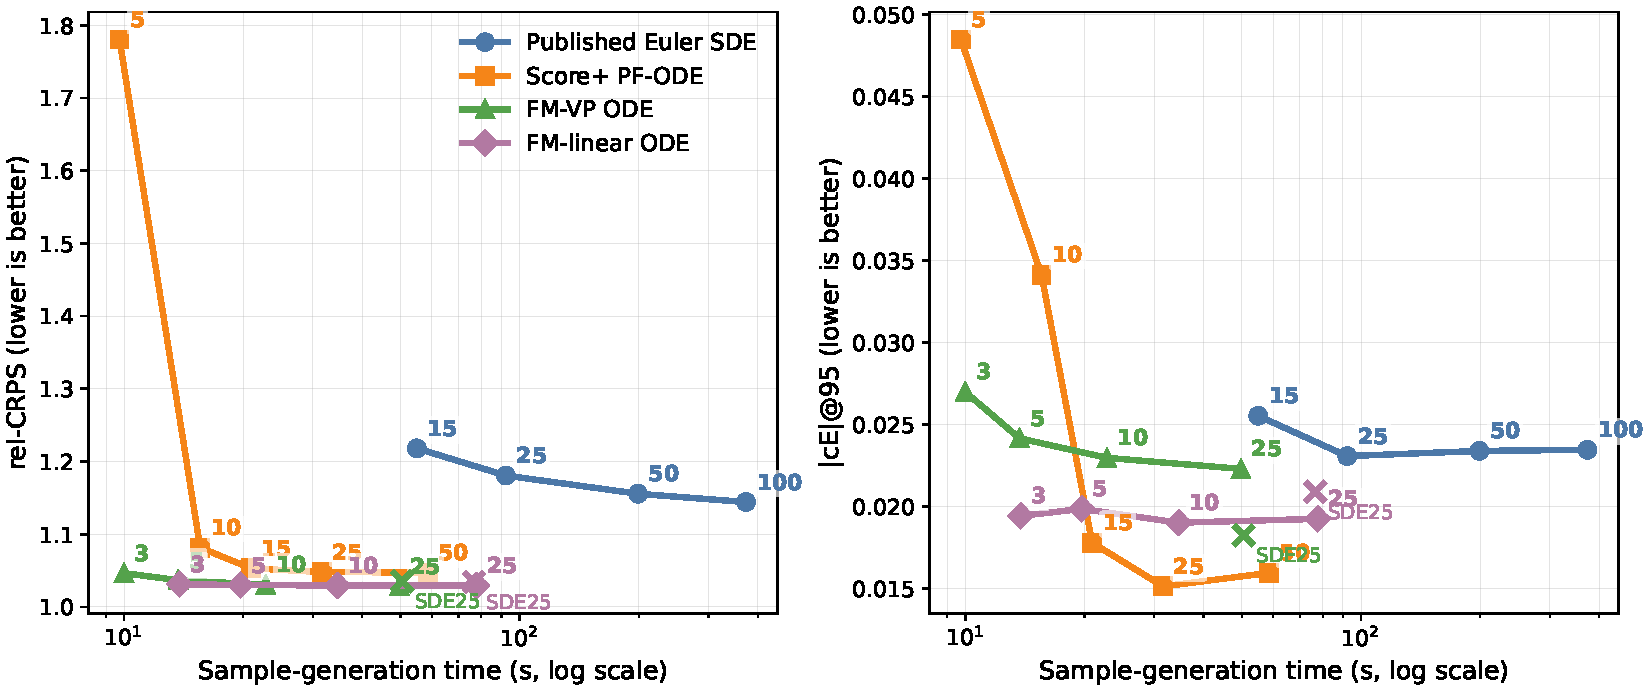
\includegraphics[width=\textwidth]{../benchmarks/results/sampler_cost_sweep/sampler_cost_tradeoff.pdf}
  \caption{Sampler cost tradeoff after tuning, averaged over the same ten UCI datasets and folds~1--5. Points are eval-only sampler changes from the tuned configurations; labels show solver steps, and \texttt{SDE25} marks the 25-step stochastic FM sampler. rel-CRPS is normalized by the best sampler-cost row on each dataset.}\label{fig:sampler-cost}
\end{figure*}

\paragraph{Design diagnostics.} Fixed diagnostics explain why particular bundles were tested, but they are not separately tuned factorial comparisons. For FM, the fixed path diagnostic in Appendix~\ref{app:path} isolates the expected feature-scale advantage of variance-preserving paths under matched residualizer-C and a 5-step Heun ODE. The tuned ablation in Table~\ref{tab:mechanism-ablation} is the performance evidence: it shows a close residualized path frontier, with linear strongest on aggregate CRPSS, trig competitive and winning two datasets, and VP fastest. Thus we treat path choice as a practical conditioning/sampling tradeoff rather than a settled hierarchy. Stochastic samplers do not Pareto-dominate $\varepsilon=0$ on aggregate CRPS/coverage/latency, though they can improve high-IQR tail coverage (Appendix~\ref{app:tail-diagnostic}); transferred score-side tricks are neutral or worse. This is why the recommendation is deterministic ODE for aggregate CRPS/latency, with stochasticity left as a conditional-calibration knob. Appendix~\ref{app:score-side} maps tuned headline claims versus fixed diagnostics.

\section{Discussion}\label{sec:disc}
Two findings deserve emphasis. First, the headline rows compare tuned bundled recipes, while Appendix~\ref{app:score-side} scopes the fixed diagnostics. Because score$^+$ and FM share the same LightGBM tuning surface, the FM result is not implicitly absorbing tuning-budget improvements that belong to the score track. Second, per-dataset tuning turns the headline into a tradeoff: score$^+$ is the strongest calibrated Treeffuser row, whereas FM is strongest on normalized CRPS and latency. The common mechanism is regression conditioning for tree ensembles: EDM preconditioning stabilises the VE score path's inputs and denoising residual, while FM changes the target and sampler geometry of the supervised problem. The tuned path ablation is important here: variance preservation is one helpful conditioning axis, but not the whole story. Linear FM has a less uniform input scale, yet its simple displacement-like velocity target and direct few-step ODE can be easier to exploit once conditional location is residualized; trig shows that the variance-preserving family remains competitive, but does not uniquely determine the CRPS optimum. Log-$\sigma$ sampling controls where tree capacity is spent, the log-$\sigma$ feature exposes the noise regime to histogram splits, residualization removes predictable conditional location, and Heun ODE sampling is an inference-side efficiency gain. The large-dataset inversion argues against a blanket ``SDE is worse'' interpretation: per-IQR-bin diagnostics show that stochasticity can improve high-uncertainty tail coverage, while aggregate metrics penalise broader intervals, worse CRPS, and higher latency.

\paragraph{Limitations.} All displayed families are tuned per dataset, but this is still finite-budget model selection with unequal search spaces and per-trial costs: the comparison is equal finite-trial budget rather than wall-clock-normalized model selection. We include six probabilistic baselines but not distributional random forests~\citep{cevid2022drf}; per-dataset gaps, especially on large datasets, should be read as descriptive rather than high-powered significance estimates. The benchmark suite is also limited to scalar UCI-style regression; categorical-heavy tables, missingness, multi-output responses, and operational tail-risk settings remain outside the evidence in this paper. The residualizer is selected from fixed diagnostics rather than automated jointly with the diffusion objective, which is the most likely reason the published SDE still wins the two largest datasets, where the inner model has enough data to fit the conditional mean directly and the fixed residualizer becomes a bottleneck.

\paragraph{Choosing a variant.} The per-dataset pattern supports benchmark-level operating points rather than a uniform-dominance claim or a simple \emph{calibration vs.\ speed} split. Use headline 5-step VP-FM when sample latency or aggregate normalized CRPS is the binding constraint; it is the fastest displayed headline corner, while the mechanism ablation shows residualized linear FM as the tuned CRPS corner and trig as a close path check. Prefer score$^+$ when interval coverage or PIT uniformity is the reported quantity, since it is the strongest calibrated row at the cost of $\sim$2.4$\times$ more sampling time. On the largest datasets, where residualizer capacity bottlenecks, the published SDE remains competitive and full SDE sampling is worth its cost. Stochasticity ($\varepsilon>0$) is a conditional knob, not a default: select it only when high-uncertainty tail coverage is the target (Appendix~\ref{app:tail-diagnostic}), against conditional-calibration metrics rather than aggregate CRPS.

\paragraph{Related uncertainty methods for trees.} Our baselines cover sample-based and quantile tree learners, but several complementary tree-uncertainty families target different quantities. Epistemic-ensemble boosting such as SGLB~\citep{ustimenko2021sglb} uses Langevin dynamics to quantify model uncertainty and is evaluated mainly on NLL/RMSE and out-of-distribution detection rather than the sharpness-and-coverage CRPS regime here. Frequentist inference for boosted trees, e.g.\ Boulevard~\citep{zhou2022boulevard}, yields asymptotic prediction intervals with coverage guarantees but does not provide a full generative predictive law. Conformal wrappers such as conformalized quantile regression~\citep{romano2019cqr} are orthogonal routes to finite-sample marginal coverage; a useful next comparison is to calibrate both Treeffuser variants and quantile-regression LightGBM under a matched calibration split and report the resulting coverage--width or interval-score tradeoff.

\paragraph{Future work.} Useful extensions include wall-clock-normalized tuning, selection criteria for stochastic samplers when conditional coverage matters, multi-output regression, and automatic residualizer selection.

\begin{ack}
Author contributions are deferred to camera-ready.
\end{ack}

\bibliography{refs}

\appendix

\section{Theoretical Derivations and Design Consequences}\label{app:theory}

\begin{lemma}[Wronskian velocity-to-score identity]\label{lem:wronskian-score}
For a differentiable Gaussian path $y_t=\alpha(t)y_0+\beta(t)z$ with conditional velocity $u_t=\alpha'(t)y_0+\beta'(t)z$, nonzero Wronskian $W(t)=\alpha(t)\beta'(t)-\alpha'(t)\beta(t)$, and $\beta(t)\neq0$ (away from the data endpoint), the population velocity $v(y_t,x,t)=\E[u_t\mid y_t,x,t]$ implies the conditional score
\[
\nabla \log p_t(y_t\mid x)=\frac{\alpha'(t)y_t-\alpha(t)v(y_t,x,t)}{W(t)\beta(t)}.
\]
\end{lemma}
\emph{Proof.} Solving the two linear equations for $z$ gives
\[
z=\frac{\alpha(t)u_t-\alpha'(t)y_t}{\alpha(t)\beta'(t)-\alpha'(t)\beta(t)}
  =\frac{\alpha(t)u_t-\alpha'(t)y_t}{W(t)}.
\]
Because $p(y_t\mid y_0,x)=\Norm(\alpha y_0,\beta^2 I)$, the conditional score is $-z/\beta(t)$. Fisher's identity gives $\nabla\log p_t(y_t\mid x)=\E[-z/\beta(t)\mid y_t,x,t]$. Substituting the expression for $z$ and using that $y_t$ is fixed under the conditional expectation yields the claim. Replacing $v$ by $v_\theta$ gives Eq.~\eqref{eq:score}. \hfill$\square$

The identity is not new theory: it specializes the standard velocity/score relations for Gaussian probability paths and stochastic interpolants~\citep{lipman2023flow,albergo2023stochastic} to the Wronskian form we use, and we present it only as the bridge that lets a velocity-trained tree model drive score-based and stochastic-interpolant samplers without retraining.

At a fixed $t$ with $\alpha(t)\neq0$, the same identity inverts to $v(y_t,x,t)=\alpha'(t)y_t/\alpha(t)-W(t)\beta(t)\nabla\log p_t(y_t\mid x)/\alpha(t)$. Thus score and velocity have the same conditional structure as functions of $y_t$ at that time; the practical differences studied here come from path-dependent scale variation across $t$, feature geometry, and sampler dynamics rather than an intrinsic fixed-$t$ smoothness advantage.

\paragraph{Path-induced feature scale.} If $y_0$ and $z$ are independent with unit variance after standardization, then the path feature satisfies
\[
\Var(y_t)=\alpha(t)^2+\beta(t)^2.
\]
Thus the linear path has $\Var(y_t)=(1-t)^2+t^2$ and compresses to variance $1/2$ at $t=1/2$, whereas the trigonometric and VP paths keep $\Var(y_t)=1$ for all $t$. This identity is elementary; its role here is to connect path choice to the empirical distribution from which histogram split candidates are built.

\begin{proposition}[Pooled histogram-bin proxy]\label{prop:histogram-bins}
Fix a scalar noised-response feature and a finite partition $\mathcal{P}=\{I_1,\ldots,I_B\}$. Let $\mathcal{H}(\mathcal{P})$ be the functions that are constant on each $I_b$, and let
\[
A_t(\mathcal{P})
=
\inf_{g\in\mathcal{H}(\mathcal{P})}
  \E_{p_t}\!\left[(f_t(y_t)-g(y_t))^2\right],
\qquad
f_t(y)=\E[T_t\mid y_t=y,x,t],
\]
where $T_t$ is the scalar score, denoising, noise, or velocity target at time $t$ with covariate value $x$ fixed. Then
\[
A_t(\mathcal{P})
\leq
\sum_{b=1}^B p_t(I_b)\,
  \operatorname{osc}_{I_b}(f_t)^2,
\]
where $\operatorname{osc}_{I_b}(f_t)=\sup_{y,y'\in I_b}|f_t(y)-f_t(y')|$. If $f_t$ is $L_t$-Lipschitz on the bins, then
\[
A_t(\mathcal{P}) \leq L_t^2\sum_{b=1}^B p_t(I_b)|I_b|^2.
\]
Moreover, in a compact-support proxy with smooth positive density $q$ and equal-$q$-mass bins $\mathcal{P}_q$, the high-resolution scaling is
\[
A_t(\mathcal{P}_q)
\lesssim
\frac{L_t^2}{B^2}\int \frac{p_t(y)}{q(y)^2}\,\dd y,
\]
up to lower-order bin-width terms.
\end{proposition}
\emph{Proof.} The best piecewise-constant approximation on a fixed partition cannot be worse than any particular constant choice on each bin. Choosing any value between the infimum and supremum of $f_t$ on $I_b$ gives pointwise squared error at most $\operatorname{osc}_{I_b}(f_t)^2$ on that bin, and integration under $p_t$ gives the first bound. The Lipschitz bound follows from $\operatorname{osc}_{I_b}(f_t)\leq L_t|I_b|$. For the high-resolution proxy, an equal-$q$-mass bin has $|I_b|\approx 1/(B q(\xi_b))$ for some $\xi_b\in I_b$, so
\[
\sum_b p_t(I_b)|I_b|^2
\approx
\sum_b p_t(\xi_b)|I_b|^3
=\frac{1}{B^2}\sum_b \frac{p_t(\xi_b)}{q(\xi_b)^3}\frac{1}{B}
\to \frac{1}{B^2}\int \frac{p_t(y)}{q(y)^2}\,\dd y,
\]
where the last step is a Riemann sum under the measure with density $q$. \hfill$\square$

\paragraph{Shared-bin mismatch.} Proposition~\ref{prop:histogram-bins} is a one-feature proxy for the finite split resolution available to a histogram tree, not a theory of the full boosted LightGBM ensemble. In the benchmark, rows from many noise levels are pooled before tree fitting, so a natural proxy is $q=\bar p$ with
\[
\bar p(y)=\int p(t)\,p_t(y)\,\dd t.
\]
The high-resolution term $\int p_t/\bar p^2$ is large when $\bar p$ allocates little bin density to regions where a particular $p_t$ still places mass. VE paths create exactly this compromise by mixing data-scale low-noise features with expanded high-noise features; a single pooled histogram must spend resolution across both regimes. EDM input preconditioning and VP-FM both reduce this mismatch by keeping the tree feature scale closer to a common range across $t$. Figure~\ref{fig:toy-preconditioning}(b) illustrates the same effect empirically: the published-style VE target is stable, but the unpreconditioned tree input expands across noise levels, whereas EDM and VP-FM keep the feature scale closer to a shared-bin regime. This is a finite-bin conditioning statement, not a claim that the fixed-time VE regression function is intrinsically rough.

\paragraph{Residualization removes predictable location.} Residualization is an exact reparameterization in the infinite-capacity limit: for any fixed $\hat\mu(x)$, modelling $r=y-\hat\mu(x)$ exactly and returning $y=r+\hat\mu(x)$ recovers the same conditional distribution. Its empirical value is finite-model conditioning. In the scalar case, if $\mu(X)=\E[Y\mid X]$ and $R=Y-\mu(X)$, the law of total variance gives
\[
\Var(Y)=\E[\Var(Y\mid X)]+\Var(\mu(X)),
\qquad
\Var(R)=\E[\Var(Y\mid X)].
\]
For vector-valued responses the same statement applies to the trace of the covariance. Thus residualization removes predictable location variation before noised responses are pooled into histogram bins. The large-dataset caveat remains: a fixed residualizer can become a bottleneck once the inner score or velocity model has enough data to represent the conditional mean directly.

\begin{proposition}[Endpoint score-error amplification]\label{prop:endpoint-amp}
Let $v_\theta(y_t,x,t)=v(y_t,x,t)+\delta(y_t,x,t)$ be an approximate velocity with pointwise error $\delta$, and let $\hat s_\theta,s$ denote the implied and true scores from Lemma~\ref{lem:wronskian-score}. Then
\[
\hat s_\theta(y_t,x,t)-s(y_t,x,t)=-\frac{\alpha(t)}{W(t)\,\beta(t)}\,\delta(y_t,x,t),
\]
so the pointwise score-error gain is $|\alpha(t)/(W(t)\beta(t))|$. For the linear and trigonometric paths, $\beta(t)\asymp t$ and $W(t)$ is bounded away from zero near $t=0$, so this gain diverges like $1/t$. For the VP path used here, $\beta(t)\asymp\sqrt{t}$ and $W(t)\asymp1/\sqrt{t}$, so $W(t)\beta(t)$ is bounded away from zero and the velocity-to-score gain remains bounded.
\end{proposition}
\emph{Proof.} Eq.~\eqref{eq:score} is linear in $v$, so
\[
\hat s_\theta - s
=\frac{\alpha'(t)y_t-\alpha(t)(v+\delta)-(\alpha'(t)y_t-\alpha(t)v)}{W(t)\beta(t)}
=-\frac{\alpha(t)\,\delta}{W(t)\beta(t)}. \tag*{$\square$}
\]

\paragraph{Endpoint amplification.} Proposition~\ref{prop:endpoint-amp} therefore predicts that any stochasticity schedule with $\varepsilon(t)\not\to 0$ as $t\to 0$ injects recovered-score error into the SDE drift. In Eq.~\eqref{eq:sde}, the recovered-score contribution to the drift error is
\[
\frac{\varepsilon(t)^2}{2}(\hat s_\theta-s)
=-\frac{\varepsilon(t)^2\alpha(t)}{2W(t)\beta(t)}\,\delta.
\]
More generally, if $\beta(t)\asymp t^a$, $\varepsilon(t)\asymp t^b$, $\alpha(t)\asymp1$, and $W(t)\asymp t^{a-1}$ near the data endpoint, this drift-error contribution scales as $t^{2b+1-2a}\delta$. Linear and trigonometric paths have $a=1$, so constant stochasticity diverges, $\varepsilon(t)\asymp\sqrt{t}$ leaves a non-vanishing endpoint error scale, and $\varepsilon(t)=ct$ makes the recovered-score contribution vanish. The VP path used here has $a=1/2$, so the velocity-to-score gain is milder, but vanishing stochasticity still suppresses the endpoint contribution and $\varepsilon\equiv0$ removes it entirely. This is why $\varepsilon(t)=ct$ and the deterministic corner are the two natural schedules in \S\ref{sec:fm}.

\paragraph{VE population identity.} On a VE path $y_t=y_0+\beta(t)z$ with $\beta'(t)>0$, normalized velocity, noise prediction, and denoising score recovery imply the same population score:
\[
s_t(y_t,x)=-\frac{\E[z\mid y_t,x,t]}{\beta(t)}
          =\frac{\E[y_0\mid y_t,x,t]-y_t}{\beta(t)^2}.
\]
Indeed, for VE, $\alpha=1$, $\alpha'=0$, $u_t=\beta'(t)z$, and $W=\beta'(t)$; Lemma~\ref{lem:wronskian-score} gives $s_t=-\E[z\mid y_t,x,t]/\beta(t)$, and $y_t=y_0+\beta(t)z$ gives the denoising form. This identity is not a claim that the finite LightGBM problems are identical. EDM fits the preconditioned denoising residual $F=(y_0-c_{\mathrm{skip}}y_t)/c_{\mathrm{out}}$ and reconstructs $D_\theta=c_{\mathrm{skip}}y_t+c_{\mathrm{out}}F_\theta$, whereas normalized VE-FM would fit $z$ directly. They imply the same score at the optimum but present different targets and feature scalings to LightGBM. This is the useful interpretation of the score$^+$--FM tie: both improve the conditioning of the regression problem seen by the tree ensemble, EDM by preconditioning the VE score objective and VP-FM by choosing a better-conditioned probability path.

\begin{table}[!h]
  \centering
  \caption{Regression-conditioning view of the main design choices. Here $y_0$ and $z$ are standardized. ``Conditioning issue'' refers to the supervised problem fit by LightGBM, not to the population score identity.}\label{tab:conditioning}
  \scriptsize
  \begin{tabular}{p{0.14\textwidth}p{0.18\textwidth}p{0.19\textwidth}p{0.29\textwidth}}
    \toprule
    Variant & Regressed object & Feature scale & Conditioning issue / fix \\
    \midrule
    VE noise prediction & $-z$ & $y_0+\sigma z$ grows with $\sigma$ & Unit target, but heteroscedastic input and $1/\sigma$ score amplification. \\
    VE EDM score$^+$ & $(y_0-c_{\mathrm{skip}}y_t)/c_{\mathrm{out}}$ & $c_{\mathrm{in}}y_t$ is near unit scale & Input and denoising residual are explicitly preconditioned. \\
    Raw VE-FM & $\beta'(t)z$ & $y_0+\beta z$ grows with $\beta$ & Velocity target inherits the schedule derivative. \\
    Normalized VE-FM & $z$ & $y_0+\beta z$ unless also scaled & Population-equivalent to noise prediction after known rescaling. \\
    VP-FM & $\alpha' y_0+\beta' z$ & $\alpha^2+\beta^2\approx1$ & Path keeps tree features near the standardized data scale. \\
    \bottomrule
  \end{tabular}
\end{table}

\begin{figure}[!h]
  \centering
  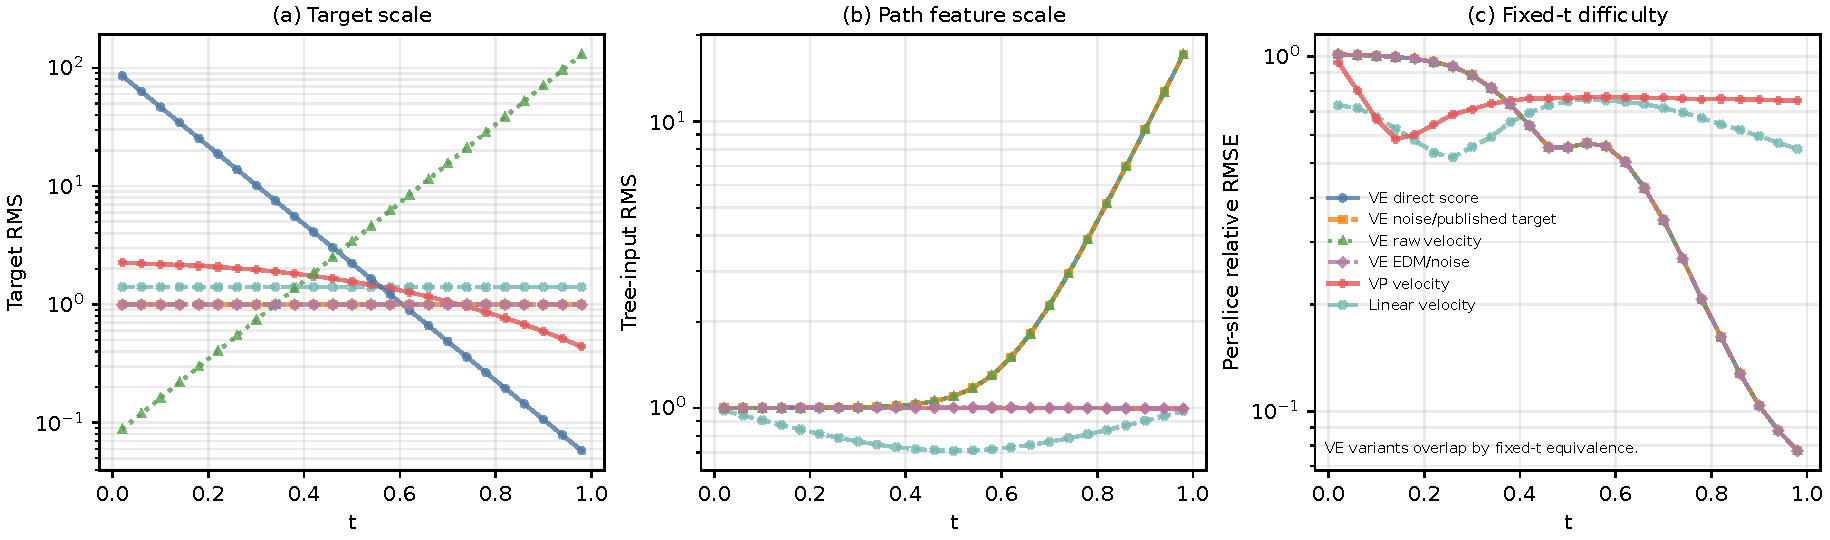
\includegraphics[width=\textwidth]{../benchmarks/results/toy_geometry_study/paper_figure.pdf}
  \caption{Toy preconditioning diagnostic on a one-dimensional heteroscedastic mixture, generated by \texttt{pixi run toy-geometry}. Panel (a) shows that direct VE score prediction and raw VE-FM have target scales that vary by orders of magnitude across $t$, whereas the published-style VE noise target, EDM/noise prediction, and linear velocity have unit target scale. Panel (b) separates target scaling from input geometry: the published-style VE target is stable but the tree input $y_t=y_0+\sigma z$ still expands strongly, while EDM rescales the input and VP-FM keeps the path feature near standardized scale. Panel (c) fits a fresh LightGBM at each fixed $t$; the VE curves overlap up to numerical noise, confirming that the score/velocity distinction is not intrinsic fixed-$t$ smoothness but cross-$t$ conditioning.}\label{fig:toy-preconditioning}
\end{figure}

\section{Datasets and Protocol Details}\label{app:datasets}

\paragraph{Sources.} The ten UCI benchmarks follow the canonical Treeffuser protocol~\citep{treeffuser}: \texttt{yacht}, \texttt{concrete}, \texttt{energy}, \texttt{wine}, \texttt{kin8nm}, \texttt{naval}, \texttt{power\_plant}, \texttt{protein} from the UCI repository; \texttt{california\_housing} from scikit-learn's \texttt{fetch\_california\_housing}; and \texttt{diabetes} from scikit-learn's \texttt{load\_diabetes}. The headline results use the six-fold tuning/evaluation protocol from \S\ref{sec:exp}; Table~\ref{tab:per-dataset} reports the post-split training rows for each evaluation fold. Fixed-configuration appendix diagnostics instead use the train/test sizes declared in their YAML configs, sometimes with large datasets subsampled for sweep cost. The only preprocessing is StandardScaler standardisation of features and target, fit on the training split and applied to the corresponding test split. \texttt{wine} is the union of \texttt{wine-quality-red} and \texttt{wine-quality-white} with a binary \texttt{color} indicator.

\paragraph{Seed policy.} The fold-tuned headline uses the deterministic six-fold manifest with master seed 0. Fixed diagnostic sweeps use the seed lists declared in their configs (usually 0--2 or 0--9), with three independent streams: \texttt{data\_seed} (offset 0) for the train/test split; \texttt{model\_seed} (offset $10{,}000$) for the LightGBM regressors; \texttt{sampler\_seed} (offset $20{,}000$) for stochastic samplers. Variance reduction across seeds therefore reflects only sampling-and-split variability, not boosting initialisation.

\paragraph{Common training settings.} In fixed diagnostic sweeps, unless noted, Treeffuser variants use $n_{\text{estimators}}=3000$, early stopping after 50 rounds, learning rate $0.1$, $n_{\text{repeats}}=30$ (each training point is reused with 30 fresh $t$ samples), and the per-output-dimension LightGBM fitter. In the headline protocol, these and other LightGBM hyperparameters are selected per dataset from the tuning spaces and stored under \texttt{benchmarks/results/tuning/best\_params/}. Inference draws 200 samples per test point.

\paragraph{Tuning budget.} For each dataset/model-family pair, Optuna targets 25 finite trials on the fold-0 train/validation split, with at most twice as many total attempts to allow failed or non-finite trials. The tuning objective is validation CRPS computed from 100 predictive Monte Carlo samples per validation point; this is the number of generated response samples used to estimate CRPS, not a subsample of validation observations. Final evaluation refits the selected configuration on each held-out evaluation fold and draws 200 samples per test point. The three Treeffuser rows share the same six-dimensional LightGBM search surface: \texttt{n\_estimators}, \texttt{learning\_rate}, \texttt{num\_leaves}, \texttt{max\_depth}, \texttt{min\_child\_samples}, and \texttt{subsample}; method-defining choices such as objective, residualization, probability path, and sampler are fixed by row. External baselines are also tuned for 25 finite trials, but their search spaces and per-trial costs differ, so the comparison should be read as equal finite-trial budget rather than wall-clock-normalized model selection. The persisted YAML files record \texttt{n\_trials\_target}, \texttt{n\_trials\_finite}, and \texttt{n\_trials\_failed}. Table~\ref{tab:tuning-spaces} summarises the per-family tunable surfaces.

\begin{table}[!h]
  \centering
  \caption{Tunable hyperparameter ranges per model family (25 Optuna trials each). Log = log-uniform sampling. Fixed method-defining parameters are not listed.}\label{tab:tuning-spaces}
  \scriptsize
  \begin{tabular}{llll}
    \toprule
    Family & Tunable parameter & Range & Scale \\
    \midrule
    Treeffuser (all 3 rows) & \texttt{n\_estimators}     & 200--3000 & log \\
                            & \texttt{learning\_rate}    & 0.001--0.3 & log \\
                            & \texttt{num\_leaves}       & 15--255 & linear \\
                            & \texttt{max\_depth}        & $\{-1, 4, 6, 8, 10\}$ & categorical \\
                            & \texttt{min\_child\_samples} & 5--100 & linear \\
                            & \texttt{subsample}         & 0.5--1.0 & linear \\
    \midrule
    NGBoost     & \texttt{n\_estimators}     & 200--3000 & log \\
                & \texttt{learning\_rate}    & 0.001--0.3 & log \\
    \midrule
    iBUG        & \texttt{k}                 & 10--200 & log \\
                & \texttt{n\_estimators}     & 200--2000 & log \\
                & \texttt{learning\_rate}    & 0.001--0.3 & log \\
                & \texttt{max\_depth}        & 3--10 & linear \\
    \midrule
    QReg-LightGBM & \texttt{quantile\_count} & 24--49 & linear \\
                   & \texttt{n\_estimators}   & 50--500 & log \\
                   & \texttt{learning\_rate}  & 0.02--0.2 & log \\
                   & \texttt{num\_leaves}     & 15--127 & linear \\
    \midrule
    CatBoost    & \texttt{iterations}        & 200--3000 & log \\
                & \texttt{learning\_rate}    & 0.001--0.3 & log \\
                & \texttt{depth}             & 4--10 & linear \\
    \midrule
    Deep ensemble & \texttt{hidden\_size}    & $\{64, 128, 256, 512\}$ & categorical \\
                  & \texttt{n\_layers}       & 2--5 & linear \\
                  & \texttt{learning\_rate}  & 0.0001--0.01 & log \\
                  & \texttt{max\_epochs}     & $\{100, 200, 400\}$ & categorical \\
    \midrule
    CARD-style  & \texttt{hidden\_size}      & $\{64, 128, 256\}$ & categorical \\
                & \texttt{n\_layers}         & 2--5 & linear \\
                & \texttt{learning\_rate}    & 0.0001--0.01 & log \\
                & \texttt{max\_epochs}       & $\{200, 400\}$ & categorical \\
                & \texttt{diffusion\_epochs} & $\{200, 400\}$ & categorical \\
                & \texttt{n\_steps}          & $\{50, 100, 200\}$ & categorical \\
    \bottomrule
  \end{tabular}
\end{table}

\paragraph{Appendix calibration metrics.} Appendix tables use $q$-MACE for sample-rank calibration: for each held-out response, we compute the fraction of predictive samples above the observed value, sort these ranks, and average their absolute deviation from an evenly spaced uniform grid. Lower $q$-MACE therefore means the sample predictive distributions have ranks closer to uniform, analogous to the PIT-KS metric in the main table but reported as an error magnitude.

\paragraph{Sampler details.}
\textsc{Treeffuser-published} uses the VESDE reverse-time SDE with the Euler--Maruyama sampler at $n_{\text{steps}}=50$, matching the published code path. \textsc{Treeffuser-score$^+$} uses the Heun probability-flow ODE at $n_{\text{steps}}=25$ steps under the EDM-style parametrization with $\sigma_{\min}=0.01$, $\sigma_{\max}=20$. \textsc{Treeffuser-FM} uses the Heun ODE at $n_{\text{steps}}=5$ on the VP path with $\beta_{\min}=0.1$, $\beta_{\max}=20$.

\section{Claim Scope and Diagnostic Cross-References}\label{app:score-side}

Unless otherwise stated, appendix sweeps are fixed-configuration diagnostics used to isolate modelling choices; they are not per-dataset tuned headline comparisons. The experimental pipeline is: fixed diagnostics identify plausible design choices; those choices define the frozen \textsc{published}, \textsc{score$^+$}, and \textsc{FM} model families; the frozen families are then tuned per dataset under the fold-0 protocol; and only that tuned protocol supports the headline aggregate performance claims.

\begin{table}[!h]
  \centering
  \caption{Scope of the empirical claims. ``Tuned'' means per-dataset Optuna selection on fold~0 before evaluation on folds~1--5; ``fixed'' means shared diagnostic settings declared in the corresponding YAML configs.}\label{tab:claim-map}
  \scriptsize
  \begin{tabular}{@{}p{0.22\textwidth}p{0.25\textwidth}p{0.17\textwidth}p{0.28\textwidth}@{}}
    \toprule
    Claim & Evidence & Tuning status & Role in the paper \\
    \midrule
    \textsc{score$^+$} and \textsc{FM} improve the Treeffuser tradeoff surface over the published row & Table~\ref{tab:headline} and Table~\ref{tab:per-dataset} & Tuned per dataset & Confirmatory performance comparison among frozen model families \\
    \textsc{score$^+$} is the most calibrated Treeffuser row under this benchmark protocol & Table~\ref{tab:headline} & Tuned per dataset & Headline aggregate calibration claim \\
    VP-FM is the preferred FM path among the tested paths & Table~\ref{tab:path} & Fixed diagnostic & Mechanism and model-selection evidence; not a claim that VP would win every independently tuned path comparison \\
    Deterministic FM is the recommended aggregate CRPS/latency sampler & Table~\ref{tab:stoch-eps} with Table~\ref{tab:tail-diagnostic} & Fixed diagnostic & Sampler diagnostic; stochasticity remains a conditional-calibration knob \\
    Residualizer-C is a reasonable headline residualizer choice & Tables~\ref{tab:off-vs-mean} and~\ref{tab:resid-AE} & Fixed diagnostic & Design choice for the frozen model families; automatic residualizer selection is left as future work \\
    Log-$\sigma$ sampling, explicit noise-level features, and EDM preconditioning motivate the \textsc{score$^+$} bundle & Toy diagnostic and development sweeps listed in Table~\ref{tab:appendix-provenance} & Fixed diagnostic & Mechanism evidence for the bundle; the quantitative performance claim is the tuned combined \textsc{score$^+$} row \\
    \bottomrule
  \end{tabular}
\end{table}

The four score-side modifications of \S\ref{sec:score-side} were validated by smoke and synthetic-core sweeps before being combined in the \textsc{score$^+$} variant.
The residualizer-C configuration that the headline uses was selected by the residualizer sweep summarised in Appendix~\ref{app:resid-config}. Log-sigma time sampling, the log-sigma noise feature, and EDM preconditioning were locked in by the \texttt{log\_sigma\_sweep}, \texttt{synthetic\_core}, and \texttt{pf\_ode\_sweep} development runs. We treat those runs as model-selection evidence rather than as separately reported tuned comparisons; the quantitative claim in the paper is the combined \textsc{score$^+$} row in Table~\ref{tab:headline}, where all four choices are evaluated together on the full ten-dataset protocol.

\section{Residualizer Configuration}\label{app:resid-config}

\subsection{Off vs.\ Mean Residualization (FM)}\label{app:off-vs-mean}

We isolate the contribution of mean residualization on the FM side at matched configuration (VP path, uniform $t$, uniform loss weighting, residualizer-C extra parameters) using a ten-dataset mixed synthetic/real diagnostic suite and ten seeds.

\begin{table}[!h]
  \centering
  \caption{FM with mean residualization vs.\ no residualization (\texttt{off}). Paired differences (mean $-$ off, 100 paired observations); negative is better for all metrics shown.}\label{tab:off-vs-mean}
  \footnotesize
  \begin{tabular}{lrrrrr}
    \toprule
    Sampler & $\Delta$CRPS & $\Delta q$-MACE & $\Delta$KS stat & $\Delta\,|\text{cE}|$@90 & paired $t$ on $\Delta$CRPS \\
    \midrule
    ODE @ 5 steps  & $-0.23$ & $-0.022$ & $-0.034$ & $-0.032$ & $-4.30$ \\
    SDE @ 25 steps & $-0.05$ & $+0.001$ & $+0.003$ & $-0.001$ & $-2.91$ \\
    \bottomrule
  \end{tabular}
\end{table}

The ODE-5 advantage is large and broadly significant across calibration metrics (81/100 paired wins on $q$-MACE and 81/100 on $|\text{cE}|$@90). At SDE-25 the gap on calibration metrics is null (paired $t<1$); the aggregate CRPS gain is driven by two real-data outliers (\texttt{yacht} $+54\%$ relative, \texttt{concrete} $+15\%$) while six of ten datasets actually favour the unresidualized baseline. The mechanism is consistent with the few-step ODE being unable to absorb the conditional mean itself when the velocity net has $\leq 5$ Heun updates; with 25 SDE updates the velocity model recovers calibration on its own. Cost: mean residualization adds $\approx 12$\,s of fit time on these sizes ($\sim 8\times$ vs.\ no residualization), so the trade is most attractive in low-step regimes.

\subsection{Residualizer Variants A--E (FM side)}\label{app:resid-AE}

Five residualizer configurations were swept on a four-dataset, three-seed sub-suite (\texttt{california\_housing}, \texttt{diabetes}, \texttt{energy}, \texttt{protein}-5k subsample) under VP-FM-ODE at 5 steps; see Table~\ref{tab:resid-AE}.

\begin{table}[!h]
  \centering
  \caption{FM residualizer diagnostic. ``Conf.\ leaves'' is the LightGBM \texttt{num\_leaves}; ``$n_{\text{est}}^{(r)}$'' is the residualizer's \texttt{n\_estimators}; ``ES'' is early-stopping rounds in the residualizer (off means no ES).}\label{tab:resid-AE}
  \footnotesize
  \begin{tabular}{llrrrrrrr}
    \toprule
    Variant & Description & Leaves & $n_{\text{est}}^{(r)}$ & ES & CRPSS $\uparrow$ & $q$-MACE $\downarrow$ & $|\text{cE}|$@95 $\downarrow$ & fit s \\
    \midrule
    A & current-baseline   & 31 & 100 & off & 0.521 & 0.028 & 0.017 & 1.82 \\
    B & regularised        & 31 & 100 & 30  & 0.509 & 0.042 & 0.018 & 2.78 \\
    C & high capacity      & 63 & 300 & off & \textbf{0.523} & 0.039 & 0.011 & 8.03 \\
    D & ES moderate        & 63 & 500 & 30  & 0.516 & 0.033 & 0.021 & 5.91 \\
    E & ES + high capacity & 63 & 2000& 30  & 0.522 & 0.034 & \textbf{0.010} & 9.81 \\
    \bottomrule
  \end{tabular}
\end{table}

Within this fixed diagnostic, configurations C and E sit on the calibration--latency Pareto front. C is the headline choice (best CRPSS, $1.2\times$ faster than E); E edges C on tail coverage ($|\text{cE}|$@95 $0.010$ vs.\ $0.011$). A separate full-protein diagnostic shows E reclaiming the lead on \texttt{protein} (CRPSS $0.476$ vs.\ C's $0.449$), reinforcing the case that the optimal residualizer is dataset-dependent.

\subsection{Scale-Aware Residualization}\label{app:mean-scale}

The \texttt{mean\_scale} residualizer additionally divides residuals by a cross-validated conditional-std estimate $\hat\sigma(x)$. On the ten-dataset mixed synthetic/real diagnostic suite with ten seeds:

\begin{table}[!h]
  \centering
  \caption{Mean vs.\ mean-scale residualization on FM at matched configuration. Higher CRPSS is better; lower CRPS, DSS, $q$-MACE are better.}\label{tab:mean-scale}
  \footnotesize
  \begin{tabular}{lrrrr}
    \toprule
    Variant & CRPSS $\uparrow$ & CRPS $\downarrow$ & DSS $\downarrow$ & $q$-MACE $\downarrow$ \\
    \midrule
    VP-FM-ODE, mean       & \textbf{0.519} & \textbf{0.652} & \textbf{$+0.314$} & \textbf{0.031} \\
    VP-FM-ODE, mean-scale & 0.489 & 0.724 & $+0.665$ & 0.038 \\
    VP-FM-SDE, mean       & \textbf{0.517} & \textbf{0.657} & \textbf{$+0.380$} & \textbf{0.040} \\
    VP-FM-SDE, mean-scale & 0.475 & 0.750 & $+0.676$ & 0.049 \\
    \bottomrule
  \end{tabular}
\end{table}

Scale-aware residualization is uniformly worse: $+11\%$ CRPS on the ODE path, $+14\%$ on the SDE path, with DSS more than doubling. The per-$x$ scale estimator is itself noisy in these finite-sample regimes; dividing by it injects more variance into the velocity target than it removes. \texttt{mean} is therefore the only residualizer carried into the headline.

\section{Time Sampling and Loss Weighting}\label{app:t-and-loss}

\subsection{Time Sampling}\label{app:t-sampling}

\begin{table}[!h]
  \centering
  \caption{FM time-sampling sweep on fixed UCI train/test splits, 10 datasets $\times$ 3 seeds, matched residualizer-C, VP path. ``uniform'' is the headline choice with an endpoint anchor at $t=1$ at probability $0.05$.}\label{tab:t-sampling}
  \footnotesize
  \begin{tabular}{lrrrrr}
    \toprule
    Variant & CRPSS $\uparrow$ & DSS $\downarrow$ & $q$-MACE $\downarrow$ & KS $p{>}.05$ $\uparrow$ & samp s \\
    \midrule
    VP-FM-ODE uniform           & \textbf{0.6564} & $-0.154$ & 0.040 & 0.47 & 3.63 \\
    VP-FM-ODE uniform anchor16  & 0.6560 & \textbf{$-0.171$} & 0.040 & 0.53 & 3.84 \\
    VP-FM-ODE logbeta           & 0.6556 & $-0.175$ & \textbf{0.035} & \textbf{0.77} & 3.74 \\
    VP-FM-ODE logSNR            & 0.6538 & $-0.135$ & 0.042 & 0.40 & 3.71 \\
    \midrule
    score$^+$ uniform-$t$       & 0.6556 & \textbf{$-0.210$} & 0.038 & 0.50 & 6.95 \\
    score$^+$ log-$\sigma$ $t$  & \textbf{0.6565} & $-0.169$ & 0.038 & \textbf{0.70} & 6.58 \\
    \bottomrule
  \end{tabular}
\end{table}

For FM, log-beta and log-SNR sampling do not move CRPS by more than $0.4\%$ relative to uniform with endpoint anchor; the smoother density shape gains $+5\%$ on KS pass rate and $-13\%$ on $q$-MACE but the effect is within seed variance for CRPSS. The headline keeps uniform-$t$ for parsimony; log-beta is a viable substitute when KS uniformity is the priority. For the score model, log-sigma sampling clearly helps PIT uniformity (KS pass $0.50 \to 0.70$) at the cost of slightly worse DSS; earlier score-side sweeps found the EDM-default $\Norm(-1.2,1.2^2)$ setting to be the safest dataset-agnostic choice among the tested log-$\sigma$ distributions. We keep log-sigma in the \textsc{score$^+$} headline because the KS gain is the more interpretable calibration win.

\subsection{Loss Weighting (min-SNR-$\gamma$)}\label{app:loss-weighting}

\begin{table}[!h]
  \centering
  \caption{Min-SNR-$\gamma$ loss weighting on FM, fixed UCI train/test splits, 10 datasets $\times$ 3 seeds. $\gamma=5$ collapses to uniform on most of the support; $\gamma=1$ amplifies the late-time loss most aggressively.}\label{tab:minsnr}
  \footnotesize
  \begin{tabular}{lrrrrr}
    \toprule
    Variant & CRPSS $\uparrow$ & CRPS $\downarrow$ & DSS $\downarrow$ & $q$-MACE $\downarrow$ & KS $p{>}.05$ $\uparrow$ \\
    \midrule
    VP-FM-ODE uniform-$w$ & \textbf{0.6564} & \textbf{4.097} & $-0.159$ & 0.040 & 0.47 \\
    VP-FM-ODE min-SNR-5   & 0.6564 & 4.119 & $-0.167$ & \textbf{0.037} & \textbf{0.60} \\
    VP-FM-ODE min-SNR-1   & 0.6516 & 4.223 & $-0.104$ & 0.044 & 0.37 \\
    VP-FM-SDE uniform-$w$ & \textbf{0.6540} & \textbf{4.114} & $-0.080$ & 0.051 & 0.30 \\
    VP-FM-SDE min-SNR-5   & 0.6538 & 4.138 & $-0.085$ & 0.050 & 0.30 \\
    VP-FM-SDE min-SNR-1   & 0.6485 & 4.239 & $-0.046$ & 0.057 & 0.23 \\
    \bottomrule
  \end{tabular}
\end{table}

Min-SNR-$\gamma$ is a sharpness-versus-tail trade-off. $\gamma=1$ hurts CRPS by $0.8$--$1.3\%$ across both samplers (Wilcoxon $p \leq 0.003$ for both); $\gamma=5$ is statistically indistinguishable from uniform weighting on CRPS, but improves PIT KS pass rate on the ODE path. We keep uniform weighting in the FM headline.

\section{Stochasticity (Velocity-Noise) Sweeps}\label{app:stoch}

\subsection{Stochasticity Strength}\label{app:stoch-eps}

We sweep velocity stochasticity on the VP path under linear and $\sqrt{t}$ schedules with residualizer-C, plus one residualizer-E check; results in Table~\ref{tab:stoch-eps} are averages over fixed UCI train/test splits, 10 datasets $\times$ 3 seeds at 25 SDE steps.

\begin{table}[!h]
  \centering
  \caption{Stochasticity sweep. The $\varepsilon=0$ corner is the deterministic FM recipe (Heun ODE @ 5 steps); SDE rows use 25 steps. Sample time is omitted because the ODE and SDE rows use different benchmark protocols.}\label{tab:stoch-eps}
  \footnotesize
  \begin{tabular}{lrrrr}
    \toprule
    Variant & CRPSS $\uparrow$ & CRPS $\downarrow$ & $|\text{cE}|$@90 $\downarrow$ & $|\text{cE}|$@95 $\downarrow$ \\
    \midrule
    $\varepsilon=0$ headline (ODE)    & 0.669 & --     & \textbf{0.024} & \textbf{0.017} \\
    $\varepsilon=0.25$ linear, res-C  & 0.656 & 4.099  & 0.028 & 0.015 \\
    $\varepsilon=0.50$ linear, res-C  & 0.655 & 4.104  & 0.036 & 0.017 \\
    $\varepsilon=1.00$ linear, res-C  & 0.654 & 4.114  & 0.047 & 0.022 \\
    $\varepsilon=0.50$ sqrt, res-C    & 0.655 & 4.101  & 0.035 & 0.017 \\
    $\varepsilon=1.00$ sqrt, res-C    & 0.655 & 4.107  & 0.043 & 0.020 \\
    $\varepsilon=1.00$ linear, res-E  & 0.651 & 4.128  & 0.048 & 0.024 \\
    \bottomrule
  \end{tabular}
\end{table}

In this fixed diagnostic sweep, no tested SDE setting Pareto-dominates $\varepsilon=0$. The closest contender ($\varepsilon=0.25$ linear) matches $|\text{cE}|$@95 ($0.015$ vs.\ $0.017$) but is strictly worse on CRPSS and $|\text{cE}|$@90, and pays $25$ SDE steps vs.\ $5$ ODE steps.

\subsection{Schedule Shape}\label{app:stoch-schedule}

The schedule $\varepsilon(t) = c\,t$ (linear) is the headline form. The $\sqrt{t}$ alternative was tested for parity at $\varepsilon \in \{0.5, 1.0\}$ and produces statistically indistinguishable CRPSS (Table~\ref{tab:stoch-eps}). Both schedules vanish at the data endpoint, which suppresses recovered-score error in the stochastic drift (Eq.~\eqref{eq:score} and Proposition~\ref{prop:endpoint-amp}); neither shape helps once $\varepsilon$ is small.

\section{Fixed Path Diagnostic}\label{app:path}

\begin{table}[!h]
  \centering
  \caption{Flow-path diagnostic under the 5-step deterministic ODE sampler: linear vs.\ trigonometric vs.\ variance-preserving, 8 datasets $\times$ 3 seeds, matched residualizer-C. Lower is better for all columns; bold is best per column.}\label{tab:path}
  \footnotesize
  \begin{tabular}{lrrrr}
    \toprule
    Path & CRPS $\downarrow$ & $q$-MACE $\downarrow$ & $|\text{cE}|$@95 $\downarrow$ & samp s \\
    \midrule
    Linear         & 4.324 & \textbf{0.026} & 0.032 & 0.49 \\
    Trigonometric  & 4.306 & 0.028 & \textbf{0.028} & \textbf{0.43} \\
    Variance-preserving (VP) & \textbf{4.294} & 0.028 & \textbf{0.028} & 0.46 \\
    \bottomrule
  \end{tabular}
\end{table}

This fixed diagnostic is meant to isolate geometry, not to select the final path. Under matched residualizer-C, a shared 5-step ODE sampler, and fixed LightGBM settings, VP is best on CRPS, while trig and VP both reduce 95\% coverage error relative to the linear path. The pattern tracks variance preservation: VP and trig satisfy $\alpha^2+\beta^2 \approx 1$, keeping $y_t$ at roughly unit scale across $t$ and stabilising the tree regressor's feature space. The tuned mechanism ablation in Table~\ref{tab:mechanism-ablation} supersedes this fixed ranking for performance claims: with per-dataset LightGBM tuning, linear has the best aggregate CRPSS, trig is competitive and wins two datasets, and VP remains fastest. We therefore read path choice as a finite-model tradeoff: variance-preserving paths stabilise feature scale, while linear FM can have a simpler displacement-like velocity target that wins CRPS after residualization and tuning.

\section{Probabilistic-Family Baselines}\label{app:competitors}

We compare the headline Treeffuser variants against six external probabilistic regressors (Table~\ref{tab:competitors}). Hyperparameters for every displayed family are selected per dataset on the same fold-0 tuning split, then evaluated on folds~1--5. The CARD row uses a compact benchmark adapter with the same two-stage conditional-mean plus conditional-diffusion structure as CARD~\citep{han2022card}, so conclusions involving CARD should be read as comparisons to this adapter rather than to a fully optimized CARD pipeline.

\begin{table}[!h]
  \centering
  \caption{Probabilistic baselines under the tuning/evaluation protocol. rel-CRPS is normalized by the best displayed variant on each dataset. Sample-time excludes fitting. The iBUG DSS is dominated by a single \texttt{wine} fold where the model assigns near-zero predictive variance to a mispredicted test point.}\label{tab:competitors}
  \scriptsize
  \begin{tabular}{lrrrrrrr}
    \toprule
    Model & CRPSS $\uparrow$ & rel-CRPS $\downarrow$ & CRPS $\downarrow$ & DSS $\downarrow$ & $q$-MACE $\downarrow$ & $|\text{cE}|$@95 $\downarrow$ & samp s \\
    \midrule
    Treeffuser-score$^+$ (ours)     & \textbf{0.681} & 1.131 & 4.057 & $-$0.214 & \textbf{0.028} & \textbf{0.015} & 34.12 \\
    Treeffuser-FM-fast (ours)       & 0.680 & \textbf{1.117} & 4.121 & \textbf{$-$0.218} & 0.034 & 0.024 & 14.41 \\
    Treeffuser-published            & 0.670 & 1.242 & 4.279 & 1.358 & 0.044 & 0.023 & 221.35 \\
    Quantile-regression LightGBM    & 0.668 & 1.459 & 4.026 & 0.016 & 0.033 & 0.044 & 0.30 \\
    Deep ensemble                   & 0.654 & 1.519 & \textbf{4.008} & 0.090 & 0.050 & 0.018 & 0.03 \\
    iBUG (XGBoost)                  & 0.649 & 1.471 & 4.193 & $1.85{\times}10^7$ & 0.069 & 0.065 & 2.89 \\
    CatBoost (uncertainty)          & 0.638 & 1.409 & 4.045 & 0.272 & 0.045 & 0.066 & \textbf{0.01} \\
    CARD-style diffusion            & 0.631 & 1.632 & 4.838 & 0.436 & 0.051 & 0.043 & 42.84 \\
    NGBoost (Gaussian)              & 0.601 & 1.550 & 4.299 & 1.957 & 0.052 & 0.101 & 0.04 \\
    \bottomrule
  \end{tabular}
\end{table}

Under this per-dataset tuning protocol, the Treeffuser variants lead on aggregate CRPSS, rel-CRPS, and coverage metrics. The external baselines are still important: deep ensembles have the best mean raw CRPS, though this scale-sensitive average is less informative about cross-dataset dominance than CRPSS or rel-CRPS, and the per-dataset winners include deep ensembles on \texttt{diabetes} and \texttt{kin8nm}, CARD on \texttt{naval}, and quantile-regression LightGBM on \texttt{protein}. Their aggregate rel-CRPS remains worse, indicating that no single tuned external family transfers as evenly across the benchmark suite as the Treeffuser variants.

\section{Extended Per-Dataset Results}\label{app:perdata-ext}

Table~\ref{tab:perdata-ext} reports CRPS, $|\text{cE}|$@90, and sample-generation time on each of the ten benchmarks for the three headline Treeffuser variants, averaged over the five evaluation folds. The ``best margin'' column gives the gap between the winning variant and the second-best Treeffuser variant in raw CRPS. After per-dataset tuning, the margins are tighter: the main result is no longer a few dramatic wins, but a more balanced Pareto surface between published SDE sampling, score-side conditioning, and FM speed.

\begin{table}[!h]
  \centering
  \caption{Extended per-dataset Treeffuser results, ordered roughly by evaluation-fold training size. ``best margin'' is winner-over-second-best in raw CRPS; the bold cell in each block is the per-metric winner on that row. Numbers come from \texttt{benchmarks/results/tuning/eval/*.jsonl}.}\label{tab:perdata-ext}
  \scriptsize
  \begin{tabular}{lrrrrrrrrrr}
    \toprule
    & & \multicolumn{3}{c}{CRPS $\downarrow$} & \multicolumn{3}{c}{$|\text{cE}|$@90 $\downarrow$} & \multicolumn{3}{c}{sample s} \\
    \cmidrule(lr){3-5} \cmidrule(lr){6-8} \cmidrule(lr){9-11}
    Dataset & best margin & Pub.\ & Score$^+$ & FM & Pub.\ & Score$^+$ & FM & Pub.\ & Score$^+$ & FM \\
    \midrule
    yacht              & FM\,$+$0.4\%      & 0.438 & 0.284 & \textbf{0.283} & 0.092 & \textbf{0.025} & 0.081 & 0.3 & 0.3 & \textbf{0.1} \\
    diabetes           & Sco$^+$\,$+$1.9\% & 35.682 & \textbf{34.025} & 34.660 & 0.079 & \textbf{0.029} & 0.038 & 2.4 & 0.5 & \textbf{0.2} \\
    energy             & FM\,$+$5.2\%      & 0.252 & 0.214 & \textbf{0.204} & 0.081 & 0.034 & \textbf{0.022} & 2.9 & 0.8 & \textbf{0.6} \\
    concrete           & Sco$^+$\,$+$1.5\% & 2.457 & \textbf{2.126} & 2.158 & 0.034 & 0.025 & \textbf{0.023} & 3.0 & 4.8 & \textbf{0.8} \\
    wine               & Pub\,$+$5.9\%     & \textbf{0.300} & 0.319 & 0.318 & 0.037 & \textbf{0.006} & 0.016 & 100.4 & 37.0 & \textbf{11.9} \\
    kin8nm             & FM\,$+$4.0\%      & 0.067 & 0.058 & \textbf{0.055} & 0.012 & \textbf{0.004} & 0.023 & 22.0 & 20.2 & \textbf{9.2} \\
    power              & FM\,$+$2.4\%      & 1.671 & 1.572 & \textbf{1.535} & 0.013 & \textbf{0.004} & 0.006 & 14.6 & \textbf{6.7} & 7.6 \\
    naval              & FM\,$+$3.2\%      & 0.000218 & 0.000220 & \textbf{0.000211} & 0.078 & 0.065 & \textbf{0.061} & 207.4 & 91.2 & \textbf{29.5} \\
    cali.\ housing     & Pub\,$+$3.6\%     & \textbf{0.197} & 0.204 & 0.206 & 0.010 & \textbf{0.005} & 0.007 & 605.9 & 52.6 & \textbf{19.2} \\
    protein            & Pub\,$+$2.7\%     & \textbf{1.722} & 1.769 & 1.796 & \textbf{0.005} & 0.005 & 0.007 & 1254.7 & 127.0 & \textbf{64.9} \\
    \bottomrule
  \end{tabular}
\end{table}

FM is the fastest Treeffuser sampler on 9/10 datasets and is especially valuable at scale: on \texttt{protein} the speedup is $19.3\times$ over \textsc{published} and $2.0\times$ over \textsc{score$^+$}; on \texttt{california\_housing} the corresponding speedups are $31.6\times$ and $2.7\times$. On $|\text{cE}|$@90, however, \textsc{score$^+$} leads on 6/10 datasets and FM on 3/10, which is why Table~\ref{tab:headline} separates normalized-CRPS and calibration conclusions. Under this evaluation protocol, the per-dataset CRPS ranking reproduces the headline pattern: FM has the best average normalized CRPS, score$^+$ is the more reliable calibration row, and the published SDE remains best on wine, california housing, and protein.

\section{Robustness by Dataset Size}\label{app:robustness}

Table~\ref{tab:robustness-size} groups the tuned evaluation artifacts by post-split training rows: small datasets have at most 1{,}000 rows, medium datasets have 1{,}001--10{,}000 rows, and large datasets have more than 10{,}000 rows. The grouping sharpens the mixed-winner story. Score$^+$ and FM lead the small and medium groups on CRPSS, while the two largest datasets favor the published SDE and quantile-regression LightGBM. Thus the aggregate Treeffuser result is not driven by a single data-scale regime, but neither does it erase the large-dataset inversion discussed in the limitations.

\begin{table}[!h]
  \centering
  \caption{Dataset-size robustness summary. Entries are mean CRPSS within each size group after first averaging the five evaluation folds per dataset.}\label{tab:robustness-size}
  \scriptsize
  \begin{tabular}{lrrr}
    \toprule
    Model & Small (4) & Medium (4) & Large (2) \\
    \midrule
    Treeffuser-published & 0.709 & 0.670 & \textbf{0.591} \\
    Treeffuser-score$^+$ & \textbf{0.735} & 0.678 & 0.578 \\
    Treeffuser-FM & 0.731 & \textbf{0.683} & 0.573 \\
    QReg-LightGBM & 0.711 & 0.666 & 0.587 \\
    CatBoost-unc. & 0.724 & 0.612 & 0.517 \\
    NGBoost & 0.718 & 0.550 & 0.468 \\
    Deep ensemble & 0.699 & 0.672 & 0.529 \\
    iBUG & 0.700 & 0.637 & 0.571 \\
    CARD-style diffusion & 0.632 & 0.667 & 0.555 \\
    \bottomrule
  \end{tabular}
\end{table}

The rank diagnostics in Table~\ref{tab:robustness-ranks} give the same guarded conclusion. The Friedman test detects differences among the nine families, but Nemenyi post-hoc comparisons at $\alpha=0.05$ only separate score$^+$ from NGBoost and FM from NGBoost/CARD-style diffusion. They do not separate FM, score$^+$, the published SDE, QReg-LightGBM, or deep ensembles from one another, so we use these ranks as robustness context rather than as a stronger significance claim.

\section{Conditional Tail Calibration Diagnostic}\label{app:tail-diagnostic}

Aggregate coverage can hide where a sampler is failing. As a lightweight conditional diagnostic, we bin held-out points by the model's predicted interquartile range (IQR) and report coverage in the highest-IQR quintile, together with IQR-MACE, the mean absolute coverage error across the five predicted-IQR bins. This is not a conditional-coverage guarantee, but it tests whether the predictive intervals behave differently on points the model itself considers uncertain. Table~\ref{tab:tail-diagnostic} uses the tuned evaluation artifacts and the sampler-cost sweep, averaging folds within each dataset and then averaging across the ten datasets.

\begin{table}[!h]
  \centering
  \caption{Conditional calibration proxy using predicted-IQR bins, averaged over the ten UCI datasets after fold averaging. Top-IQR Cov@$q$ is empirical coverage in the highest predicted-IQR quintile; IQR-MACE@$q$ is mean absolute coverage error across all five predicted-IQR bins. FM-SDE rows are eval-only sampler changes from the tuned FM configurations.}\label{tab:tail-diagnostic}
  \scriptsize
  \begin{tabular}{lrrrrr}
    \toprule
    Row & Top-IQR Cov@90 & IQR-MACE@90 & Top-IQR Cov@95 & IQR-MACE@95 & $|\text{cE}|$@95 \\
    \midrule
    Published Euler-50 & 0.927 & 0.053 & 0.961 & 0.030 & 0.023 \\
    Score$^+$ PF-ODE-25 & 0.880 & \textbf{0.042} & 0.932 & 0.031 & \textbf{0.015} \\
    FM-VP ODE-5 & 0.854 & 0.051 & 0.906 & 0.040 & 0.024 \\
    FM-VP SDE-25 & \textbf{0.902} & 0.050 & \textbf{0.944} & \textbf{0.030} & 0.018 \\
    FM-linear ODE-5 & 0.848 & 0.048 & 0.902 & 0.035 & 0.020 \\
    FM-linear SDE-25 & 0.891 & 0.053 & 0.935 & 0.034 & 0.021 \\
    \bottomrule
  \end{tabular}
\end{table}

The diagnostic supports a tradeoff rather than a one-sided conclusion. Deterministic FM under-covers the most uncertain quintile at 95\% nominal coverage: 0.906 for VP and 0.902 for linear. Adding stochasticity lifts those numbers to 0.944 and 0.935, respectively, and improves VP's IQR-MACE@95 from 0.040 to 0.030. However, the same SDE rows require 25 stochastic steps and, as Figure~\ref{fig:sampler-cost} shows, are not the aggregate CRPS/latency default. The published SDE and score$^+$ remain competitive on this diagnostic, so the safest interpretation is that stochastic FM is a useful conditional-calibration option, not a uniformly better sampler.

\section{Reproducibility}\label{app:repro}

The submission includes an anonymized frozen repository via \texttt{anonymous.4open.science}. The repository contains the implementation in \texttt{src/}, the benchmark harness in \texttt{benchmarks/}, the paper sources in \texttt{paper/}, and the \texttt{pixi.toml}/\texttt{pixi.lock} environment used for the reported runs. All sweeps in this paper are driven by YAML configs under \texttt{benchmarks/configs/}. Each result file is a JSON Lines document recording the full hyperparameter set, random seeds, the git commit hash of the model code, a hash of the Treeffuser source tree, and every reported metric on a per-dataset/per-fold row. The headline tuning runs persist their selected configurations under \texttt{benchmarks/results/tuning/best\_params/} and their five-fold evaluation rows under \texttt{benchmarks/results/tuning/eval/}. The configs and result artifacts that produced the tables are listed alongside in Table~\ref{tab:appendix-provenance}; the paper PDF is rebuilt with the \texttt{paper} pixi task.

\begin{table}[!h]
  \centering
  \caption{Provenance: appendix tables and the config / result file each was produced from.}\label{tab:appendix-provenance}
  \scriptsize
  \resizebox{\textwidth}{!}{%
  \begin{tabular}{lll}
    \toprule
    Table & Config & Result file \\
    \midrule
    \ref{tab:off-vs-mean}   & \texttt{fm\_off\_vs\_mean\_sweep.yaml}   & \texttt{fm\_off\_vs\_mean\_sweep\_\_*.jsonl} \\
    \ref{tab:conditioning}   & analytic summary & -- \\
    \ref{tab:resid-AE}      & \texttt{residualizer\_fm\_sweep.yaml}    & \texttt{residualizer\_fm\_sweep\_\_*.jsonl} \\
    \ref{tab:mean-scale}    & \texttt{fm\_mean\_scale\_sweep.yaml}     & \texttt{fm\_mean\_scale\_sweep\_\_*.jsonl} \\
    \ref{tab:t-sampling}    & \texttt{fm\_t\_sampling\_sweep.yaml}     & \texttt{fm\_t\_sampling\_sweep\_\_*.jsonl} \\
    \ref{tab:minsnr}        & \texttt{fm\_loss\_weighting\_sweep.yaml} & \texttt{fm\_loss\_weighting\_sweep\_\_*.jsonl} \\
    \ref{tab:stoch-eps}     & \texttt{sde\_lower\_stoch\_sweep.yaml}, \texttt{stochasticity\_schedule\_sweep.yaml} & \texttt{sde\_lower\_stoch\_sweep\_\_*.jsonl}, \texttt{stochasticity\_schedule\_sweep\_\_*.jsonl} \\
    \ref{tab:path}          & \texttt{ode\_vs\_sde\_path\_ablation.yaml}          & \texttt{ode\_vs\_sde\_path\_ablation\_\_*.jsonl} \\
    \ref{tab:competitors}, \ref{tab:per-dataset}, \ref{tab:perdata-ext}, \ref{tab:headline} & \texttt{tuning\_manifest.yaml} & \texttt{benchmarks/results/tuning/eval/*.jsonl} \\
    \ref{tab:robustness-ranks}, \ref{tab:robustness-size} & \texttt{benchmarks/scripts/summarize\_robustness.py} & \texttt{benchmarks/results/selected/robustness\_summary.md} \\
    \ref{tab:mechanism-ablation} & \texttt{mechanism\_ablation\_manifest.yaml} & \texttt{benchmarks/results/mechanism\_ablation/eval/*.jsonl} \\
    \ref{fig:sampler-cost}, \ref{tab:tail-diagnostic} & \texttt{benchmarks/scripts/run\_sampler\_cost\_sweep.py}, \texttt{benchmarks/scripts/summarize\_sampler\_cost\_sweep.py} & \texttt{benchmarks/results/sampler\_cost\_sweep/eval/sampler\_cost\_sweep.jsonl} \\
    \ref{tab:tuning-spaces} & \texttt{benchmarks/tuning/search\_spaces.py} & -- \\
    \bottomrule
  \end{tabular}}
\end{table}

\newpage
\input{checklist.tex}

\end{document}
